\chapter{Metodologia}
\label{cap:metodologia}

Este capítulo descreve a abordagem metodológica adotada, composta por três elementos principais: uma Revisão Sistemática da Literatura (detalhada no Apêndice A), um \textit{survey} exploratório (cujos resultados completos estão no Apêndice B) e a Design Science Research (DSR) para o desenvolvimento do artefato proposto.

A análise dos logs coletados assumiu caráter exploratório \cite{gil2018metodos}, uma vez que não partiu de categorias pré-definidas, mas buscou identificar padrões emergentes de uso de palavras reservadas, lacuna evidenciada pela Revisão Sistemática. O processo de agrupamento foi conduzido de forma não supervisionada, com documentação sistemática das decisões analíticas para garantir transparência e reprodutibilidade. Esta abordagem está alinhada aos princípios da Descoberta de Conhecimento em Bases de Dados (KDD) \cite{fayyad1996knowledge} e à área de Mineração de Dados Educacionais \cite{baker2009state}.

\section{Abordagem Metodológica}

Este trabalho foi conduzido no Instituto Federal de Educação, Ciência e Tecnologia do Amazonas, Campus Avançado Boca do Acre, utilizando uma abordagem metodológica mista. Foram combinados métodos de pesquisa bibliográfica e empírica para fundamentar o trabalho tanto no estado da arte quanto no contexto prático do problema investigado. Os procedimentos metodológicos da pesquisa respeitaram os preceitos éticos que regem pesquisas com seres humanos.\subsection{Revisão Sistemática da Literatura}
%\label{subsec:revisao-sistematica}

Para mapear o estado da arte sobre o uso de logs no ensino de programação, foi conduzida uma Revisão Sistemática da Literatura (RSL) seguindo as diretrizes atualizadas para revisões sistemáticas em Engenharia de Software, incluindo o guia SEGRESS \cite{kitchenham2023segress} e o protocolo PRISMA 2020 \cite{page2021prisma}.

\subsection{Survey Exploratório}
%\label{subsec:survey}

Complementarmente à RSL, foi realizado um \textit{survey} com 14 participantes (docentes, mestrandos em computação e pesquisadores da área de ensino de programação) com o objetivo de investigar o uso de ferramentas de captura de logs, construção de avaliações quantitativas e desenvolvimento de \textit{datasets} acadêmicos. O instrumento de coleta continha 10 questões abordando logs, uso de ferramentas e IDEs. As respostas completas do \textit{survey} e a análise detalhada encontram-se no \textbf{Apêndice B}.

\subsection{Design Science Research}
\label{subsec:dsr}

Este trabalho adotou a abordagem de Design Science Research (DSR), conforme os paradigmas fundacionais propostos por \cite{hevner2004design} e \cite{peffers2007design}. Mais recentemente, \cite{hevner2024transparency} destacam que a transparência deve ser endereçada ao longo de todo o projeto de DSR, desde o planejamento até a disseminação dos resultados, alinhando-se aos princípios de design aberto e ciência aberta.

A presente pesquisa incorpora esses princípios de três formas: (i) o plugin LOGADO é disponibilizado publicamente no GitHub sob licença MIT; (ii) os logs coletados são visíveis e acessíveis ao estudante; (iii) as decisões de projeto e análise são documentadas de forma sistemática nesta dissertação.

O processo de DSR foi executado em quatro atividades principais:

\subsubsection{Atividade 1: Identificação do Problema e Motivação}

O problema central identificado foi a carência de ferramentas específicas para captura e análise de logs acadêmicos no ensino de programação. Essa lacuna é particularmente relevante no contexto da região Amazônica, onde instituições como o Instituto Federal do Amazonas (IFAM) vêm sendo implantadas por meio de políticas públicas de interiorização do ensino. A criação de campi avançados, como o de Boca do Acre, representa um esforço de levar educação profissional e tecnológica a regiões historicamente desassistidas. Nesse cenário, a produção de pesquisa aplicada e o desenvolvimento de soluções tecnológicas locais são formas de demonstrar os resultados concretos dessas políticas, mostrando que é possível gerar conhecimento de qualidade também fora dos grandes centros urbanos. A falta de ferramentas adequadas para coleta e análise de logs, no entanto, limita a capacidade dessas instituições de identificar dificuldades de aprendizagem de forma objetiva e baseada em dados.

\subsubsection{Atividade 2: Definição dos Objetivos da Solução}

Com base no problema identificado e no contexto institucional da pesquisa (um campus avançado do IFAM na região Amazônica), definiram-se os seguintes objetivos:

\textbf{Objetivo Geral:} Desenvolver e validar um plugin para coleta e análise de logs durante o processo de ensino-aprendizagem de programação, demonstrando que é possível produzir soluções tecnológicas de qualidade também em contextos de interiorização do ensino.

\textbf{Objetivos Específicos:}
\begin{enumerate}
    \item Projetar e implementar um plugin de captura de eventos integrado à IDE adotada na disciplina.
    \item Estabelecer um procedimento de coleta, sincronização e armazenamento dos dados gerados.
    \item Estruturar os logs coletados em um dataset organizado e documentado.
    \item Avaliar a viabilidade da abordagem por meio da coleta de dados em contexto real de sala de aula.
\end{enumerate}

\subsubsection{Atividade 3: Design e Desenvolvimento}

O design e desenvolvimento seguiu uma abordagem iterativa, com ajustes contínuos durante as atividades práticas da disciplina. A arquitetura do artefato compreende quatro módulos principais:

\begin{itemize}
    \item Módulo de captura: coleta palavras reservadas e timestamps.
    \item Módulo de estruturação: organiza os eventos em JSON.
    \item Módulo de armazenamento: gerencia os arquivos localmente.
    \item Módulo de configuração: permite verificar se a extensão está ativa e coletando logs corretamente.
\end{itemize}

\subsubsection{Especificação de Requisitos do Artefato}
%\label{subsubsec:requisitos}

Para garantir que o \textit{plugin} LOGADO atendesse aos objetivos da pesquisa e às necessidades dos usuários finais, foi realizada uma etapa de especificação de requisitos. A análise inicial identificou dois atores principais, cujas necessidades são sumarizadas na Tabela \ref{tab:analise-atores}.

\begin{table}[h!]
\centering
\caption{Análise de atores e necessidades do sistema}
\label{tab:analise-atores}
\begin{tabular}{|p{0.3\linewidth}|p{0.3\linewidth}|p{0.3\linewidth}|}
\hline
\textbf{Ação} & \textbf{Discente} & \textbf{Pesquisador} \\
\hline
Funções necessárias & Enviar dados de execução & Desenvolver/testar plugin \\
\hline
Necessidade principal & Instalar e usar o plugin & Validar processamento de logs \\
\hline
Operações CRUD & Enviar (criar) logs & Gerenciar usuários e dataset \\
\hline
\end{tabular}
\end{table}

Com base nesta análise, foram elaborados diagramas de casos de uso para especificar as funcionalidades do sistema. A Figura \ref{fig:casos-uso-discente} ilustra as interações do ator Discente, enquanto a Figura \ref{fig:casos-de-usos-pesquisa} detalha as funcionalidades para o Pesquisador.

\begin{figure}[H]
    \centering
    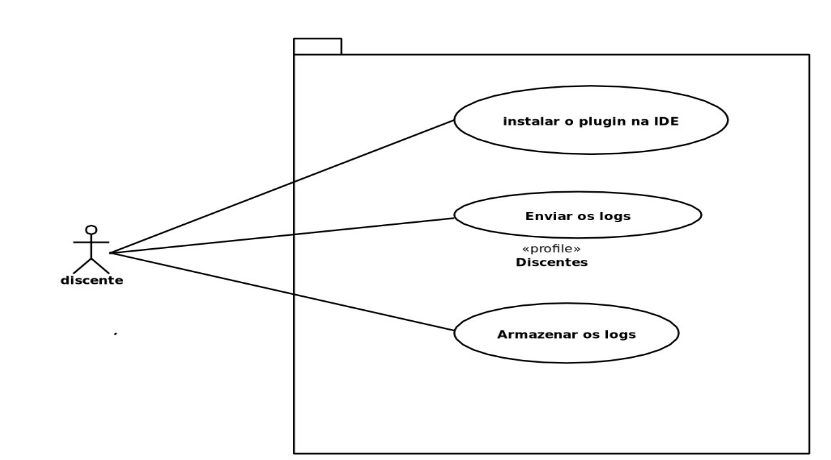
\includegraphics[width=1.1\textwidth]{../figuras/caso-de-uso-discentes.png}
    \caption{Casos de uso do \textit{plugin} LOGADO - Visão do Discente}
    \label{fig:casos-uso-discente}
\end{figure}

\begin{figure}[H]
    \centering
    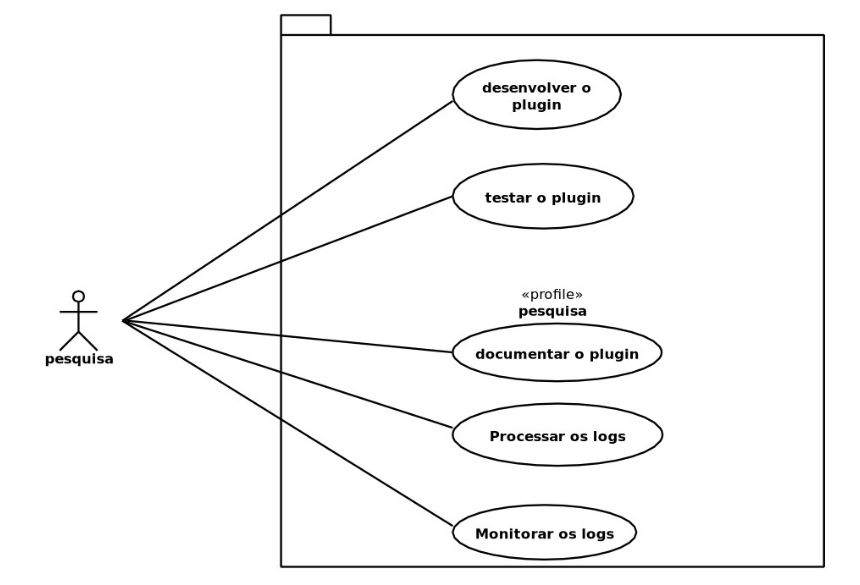
\includegraphics[width=1.1\textwidth]{../figuras/caso-de-uso-pesquisa.png}
    \caption{Casos de uso do \textit{plugin} LOGADO - Visão do Pesquisador}
    \label{fig:casos-de-usos-pesquisa}
\end{figure}

A partir dos casos de uso, foram derivados os requisitos formais do sistema:

\paragraph{Requisitos Funcionais}
Os requisitos funcionais definem as funcionalidades que o sistema deve executar. Para o ator \textbf{Discente}, o \textit{plugin} deve:
\begin{itemize}
    \item \textbf{RF01:} Registrar automaticamente eventos de edição de código (ex.: inserção, deleção de caracteres).
    \item \textbf{RF02:} Capturar eventos de compilação e execução de código, incluindo sucesso ou falha.
    \item \textbf{RF03:} Armazenar localmente os logs com \textit{timestamp} preciso.
    \item \textbf{RF04:} Transmitir os logs anonimizados para um servidor remoto de forma assíncrona.
    \item \textbf{RF05:} Exibir notificações de confirmação de operações para o usuário.
\end{itemize}

Para o ator \textbf{Pesquisador}, o \textit{plugin} deve:
\begin{itemize}
    \item \textbf{RF06:} Fornecer uma interface de configuração para parametrizar os eventos a serem capturados.
    \item \textbf{RF07:} Gerar identificadores únicos anônimos para cada sessão de uso.
\end{itemize}

\paragraph{Requisitos Não-Funcionais}
Estes requisitos definem os critérios de qualidade para o sistema:
\begin{itemize}
    \item \textbf{RNF01 (Desempenho):} O \textit{plugin} não deve impactar significativamente o desempenho da IDE. O tempo de resposta deve ser inferior a 100ms para operações de registro.
    \item \textbf{RNF02 (Usabilidade):} A instalação e o uso devem ser simples, não requerendo configuração complexa por parte do discente.
    \item \textbf{RNF03 (Confiabilidade):} O \textit{plugin} deve garantir a persistência dos logs mesmo em caso de fechamento inesperado da IDE.
    \item \textbf{RNF04 (Segurança e Privacidade):} Todos os dados pessoais devem ser anonimizados antes do envio ao servidor, conforme a LGPD.
\end{itemize}

\paragraph{Desenvolvimento do Artefato}
Foi desenvolvido um \textit{plugin} chamado LOGADO para o Visual Studio Code, com funcionalidades de captura de eventos de programação.

\subsubsection{Atividade 4: Demonstração e Avaliação}

\paragraph{Contexto e Participantes}
A pesquisa foi realizada no IFAM Campus Avançado Boca do Acre. Participaram 23 estudantes do curso técnico em Informática, de um total de 25 que assinaram o Termo de Consentimento Livre e Esclarecido (TCLE).

\paragraph{Procedimentos de Coleta}
\begin{itemize}
    \item Duração: 5 semanas de aulas práticas.
    \item Local: Laboratório de Informática do campus.
    \item Ferramenta: Visual Studio Code com a extensão LOGADO instalada.
    \item Aspectos éticos: Aprovação do Comitê de Ética e aplicação do TCLE.
\end{itemize}

\paragraph{Avaliação do Artefato}
A avaliação da extensão LOGADO foi conduzida em duas frentes: (i) verificação da integridade e completude dos logs gerados durante as atividades; (ii) análise da percepção dos estudantes sobre a transparência e o impacto da ferramenta em seu processo de aprendizagem, coletada por meio de um survey ao final do período de coleta (Apêndice B).

\section{Plano de Análise de Dados}
\label{sec:analise-dados}

Os dados coletados foram analisados nas seguintes etapas:

\subsection{Pré-processamento e Limpeza}\label{subsec:limpeza}

Os estudantes participantes, após assinatura do Termo de Consentimento Livre e Esclarecido (TCLE), tiveram a opção de submeter voluntariamente seus códigos e os arquivos JSON gerados pela extensão LOGADO a um repositório público no GitHub. Para automatizar o processo de coleta desses dados, foi desenvolvido um script que:
\begin{itemize}
    \item acessa o repositório e baixa os arquivos submetidos;
    \item organiza os logs em diretórios separados por estudante;
    \item anonimiza os dados, substituindo identificadores pessoais por códigos numéricos, em conformidade com a LGPD.
\end{itemize}

Após o download e a anonimização, os logs brutos foram submetidos a um processo de filtragem para remoção de entradas duplicadas ou inconsistentes.

\subsection{Análise Exploratória e Identificação de Padrões}
\label{subsec:identificacoes-padroes}

A análise dos logs coletados assumiu caráter exploratório \cite{gil2018metodos}, uma vez que não partiu de categorias pré-definidas, mas buscou identificar padrões emergentes de uso de palavras reservadas, lacuna evidenciada pela Revisão Sistemática (Seção \ref{subsec:revisao-sistematica}).

Os dados gerados por este trabalho constituem uma base que pode, em pesquisas futuras, ser submetida a técnicas da Descoberta de Conhecimento em Bases de Dados (KDD) \cite{fayyad1996knowledge} e da Mineração de Dados Educacionais \cite{baker2009state}. Neste estudo, contudo, o foco recaiu sobre a análise exploratória descritiva, identificando padrões a partir da observação direta dos logs.

\subsection{Potencial do Dataset e Possibilidades de Análise}
\label{subsec:potencial-possibilidades}

O dataset gerado a partir da coleta de logs abre possibilidades para investigações futuras sobre padrões de aprendizagem em programação. Com base nos dados coletados, é possível vislumbrar análises como:
\begin{itemize}
    \item sequências de declaração de variáveis (ex.: múltiplos \texttt{let} consecutivos);
    \item transições conceituais (ex.: mudança de \texttt{let} para \texttt{var} em diferentes escopos);
    \item sincronia temporal entre estudantes, possivelmente refletindo dinâmicas de mediação pedagógica;
    \item associações entre palavras-chave e desempenho acadêmico.
\end{itemize}

Não é objetivo deste trabalho esgotar essas análises, mas sim disponibilizar os dados para que outros pesquisadores possam realizá-las. O foco da presente pesquisa recai sobre o desenvolvimento do plugin LOGADO, a experiência de coleta no IFAM Campus Avançado Boca do Acre e a participação voluntária de estudantes de nível técnico em uma pesquisa de mestrado, demonstrando que é possível produzir ciência e tecnologia de qualidade também em contextos de interiorização do ensino.

\section{Percurso de Execução da Pesquisa}
\label{sec:percurso-execucao}

As atividades previstas no cronograma da pesquisa foram executadas ao longo do período de mestrado, com os seguintes marcos alcançados:

\begin{itemize}
    \item \textbf{Desenvolvimento do plugin}: extensão LOGADO implementada na versão \texttt{0.0.5}, disponível para instalação via arquivo \texttt{.vsix};
    \item \textbf{Coleta de dados}: realizada com 25 estudantes que assinaram o TCLE, com participação efetiva de 23 ao longo de 5 semanas, totalizando 19 repositórios;
    \item \textbf{Publicação associada}: uma versão preliminar do trabalho foi aceita para apresentação na LACLO (Conferência Latinoamericana de Tecnologias de Aprendizagem). O capítulo completo foi posteriormente publicado em livro pela Springer, disponível em: \url{https://link.springer.com/book/10.1007/978-981-95-7580-0}.
\end{itemize}

A pesquisa respeitou os preceitos éticos da Resolução n° 510 de 2016.